\section{\review{Chromaticity}}


% --------------------------------
%         Procedure
% --------------------------------
\subsection{\review{Procedure}}
\label{subsection:decapoles:chromaticity:measurement}

As described in \cref{subsection:optics_corrections_chromaticity}, the momentum offset $\delta$ is
related to the RF frequency and the momentum compaction factor. This relation is given as a
simplified form in \cref{eq:very_high_orders:simplified_eq_momentum_compaction}. 
The model $\alpha_c$ for the LHC injection optics is $3.48 \times 10^{-4}$ for beam 1 and $3.47
\times 10^{-4}$ for beam 2.  Via this relation, a change of 140Hz of the RF frequency corresponds to
a momentum offset of about $-0.001$.

\begin{equation}
    \delta = -\frac{1}{\alpha_c} \cdot \frac{\Delta f_{RF}}{f_{RF,nominal}}.
    \label{eq:very_high_orders:simplified_eq_momentum_compaction}
\end{equation}

%The standard measurement procedure is to vary the RF frequency to induce a change in momentum
%offset. Frequency steps of 20Hz are taken roughly every 30 seconds, to allow for a precise tune
%measurement. Once beam losses, registered by the beam loss monitors (BLM), are deemed too high the
%frequency is reverted back to its nominal frequency in larger steps. \cref{rf_scan} shows a typical
%RF scan performed to measure chromaticity.
%
%\begin{figure}[tbh]
%    \centering
%    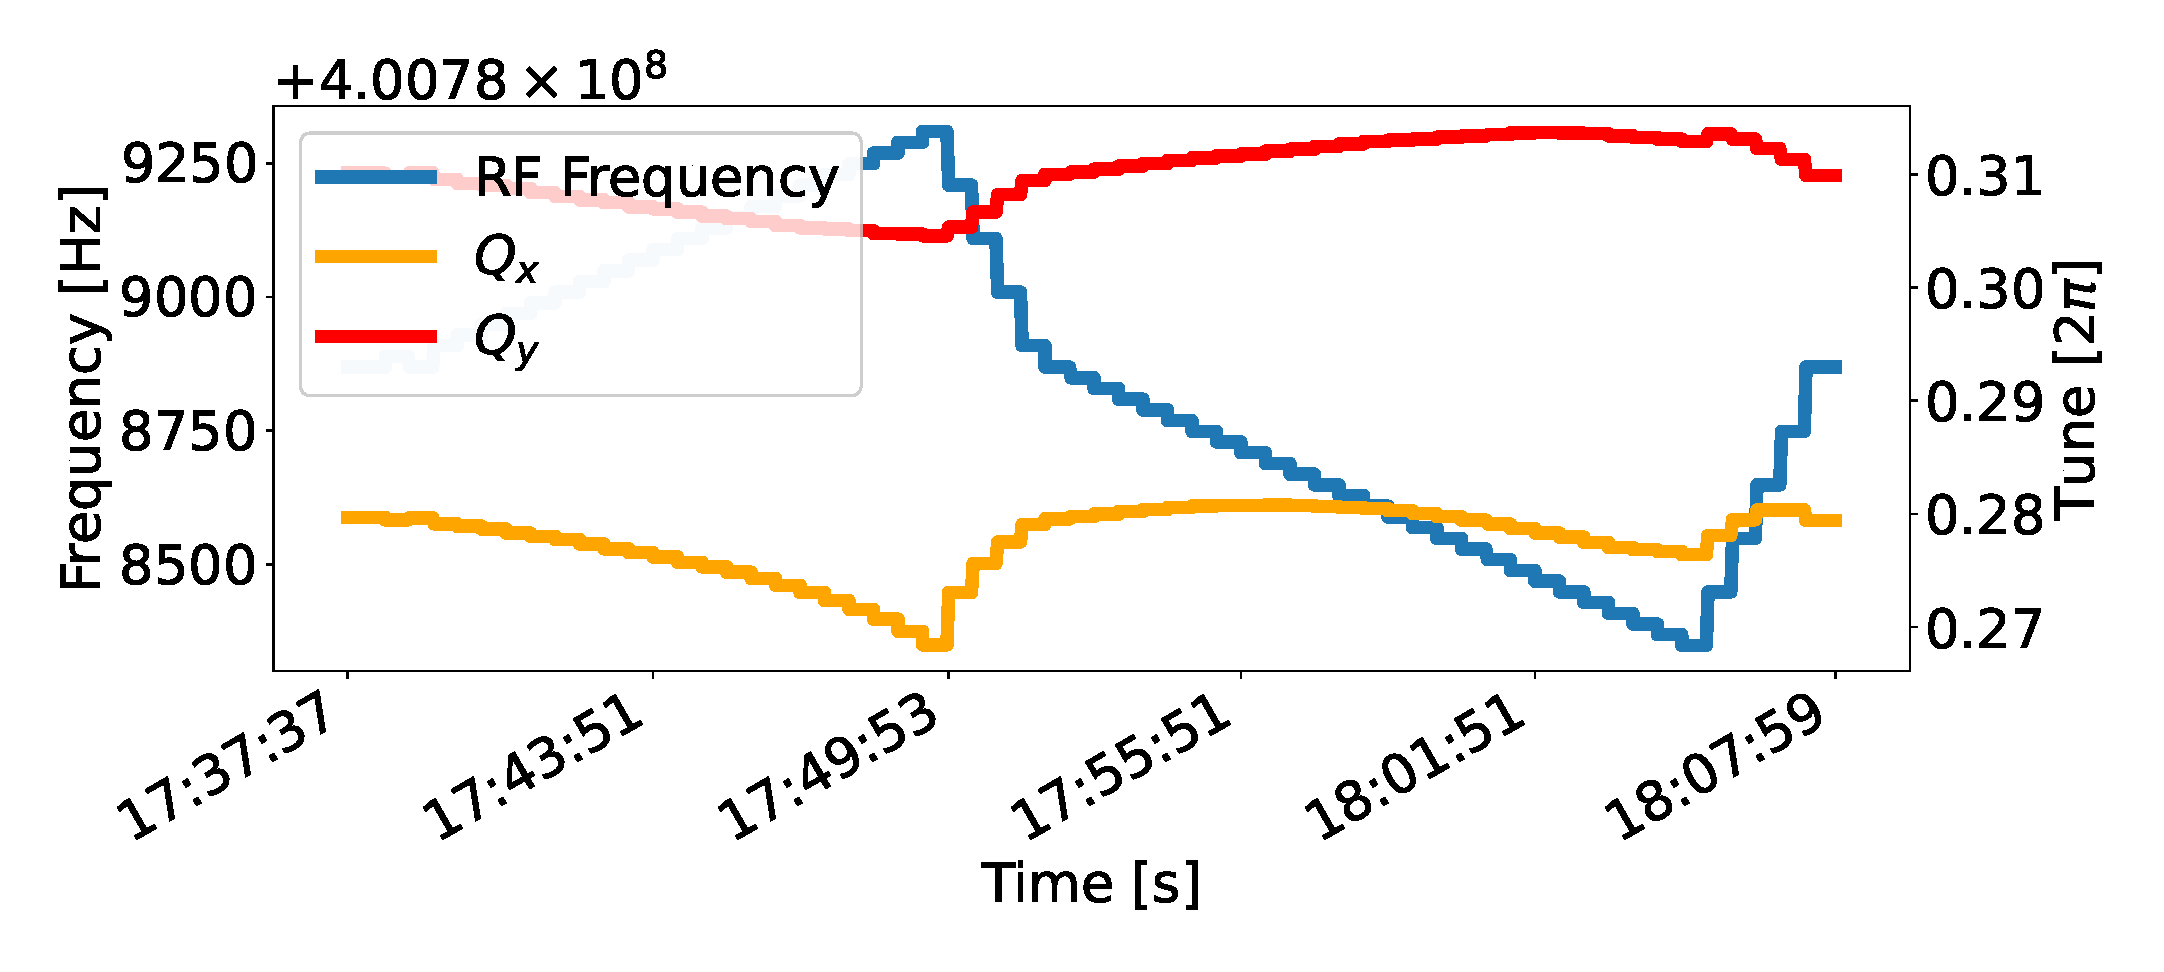
\includegraphics[width=\columnwidth]{images/MOPL027_f1-1.pdf}
%    \caption{Observation of the tune dependence on momentum offset, created by a shift of RF frequency.}
%    \label{rf_scan}
%\end{figure}

To properly characterize higher orders of the chromaticity function and ensure quality measurements,
several steps are required. The tune measured during chromaticity scans can exhibit jitter and
resonance lines may appear, requiring thorough data cleaning to either reject problematic data
points or reduce error bars. The simplified
\cref{eq:very_high_orders:simplified_eq_momentum_compaction}, describing $\delta$, has been
sufficient for reliably measuring up to the third order chromaticity. However, this relation also
needs verification.




% ========== Noisy Tune
\subsubsection{\review{Noise and Spectral Lines}}

Noise lines, due to electronics, can be seen in the raw data obtained from the BBQ tune system.
Occasionally, when those resonances are strong, their frequency peak can be mistaken as the tune and
logged as such by the system. This yield large uncertainties in the measurement when data points 
can't properly be classified as outliers. A tune measurement presenting this issue is showed in 
\cref{fig:decapoles:chromaticity:noisy_tune}.

\begin{figure}[H]
    \centering
    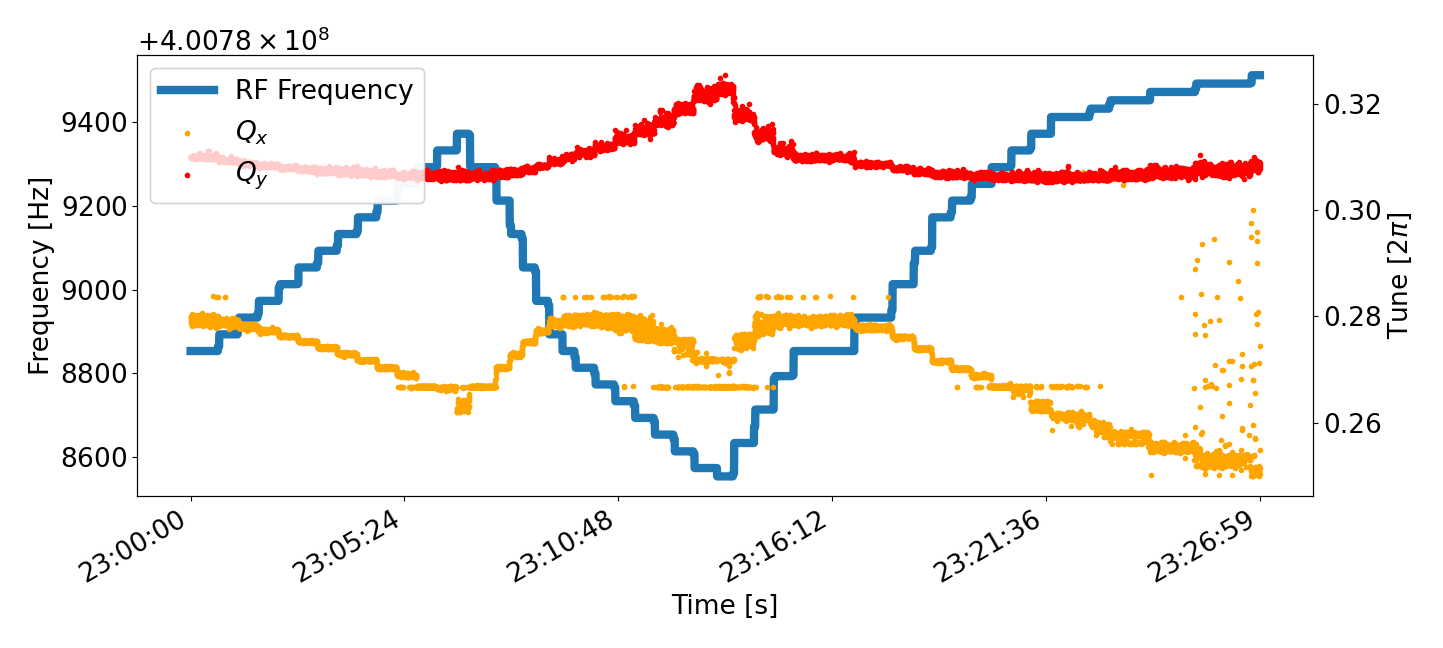
\includegraphics[width=\textwidth]{./images/noisy_tune.png}
    \caption{Shift of the tune by variation of the RF. Noise lines can appear in some cases,
    making the tune error bar large or downright unusable.}
    \label{fig:decapoles:chromaticity:noisy_tune}
\end{figure}

A solution to this issue is to use the raw data extracted from the BBQ system. From there, a
spectrogram clearly shows the noise lines, as seen in \cref{fig:decapoles:chromaticity:spectrogram}.
Those lines have been repeatedly identified over several measurements and confirmed to be fixed.
The highest peak of the spectrogram can thus be safely identified by removing those resonances,
yielding a cleaner measurement. It is also to be added that the BBQ requires to set a tune window,
which can be forgotten. By analyzing the raw data, it is ensured that the measurement has usable
data and does not try to measure noise.

\begin{figure}[H]
    \centering
    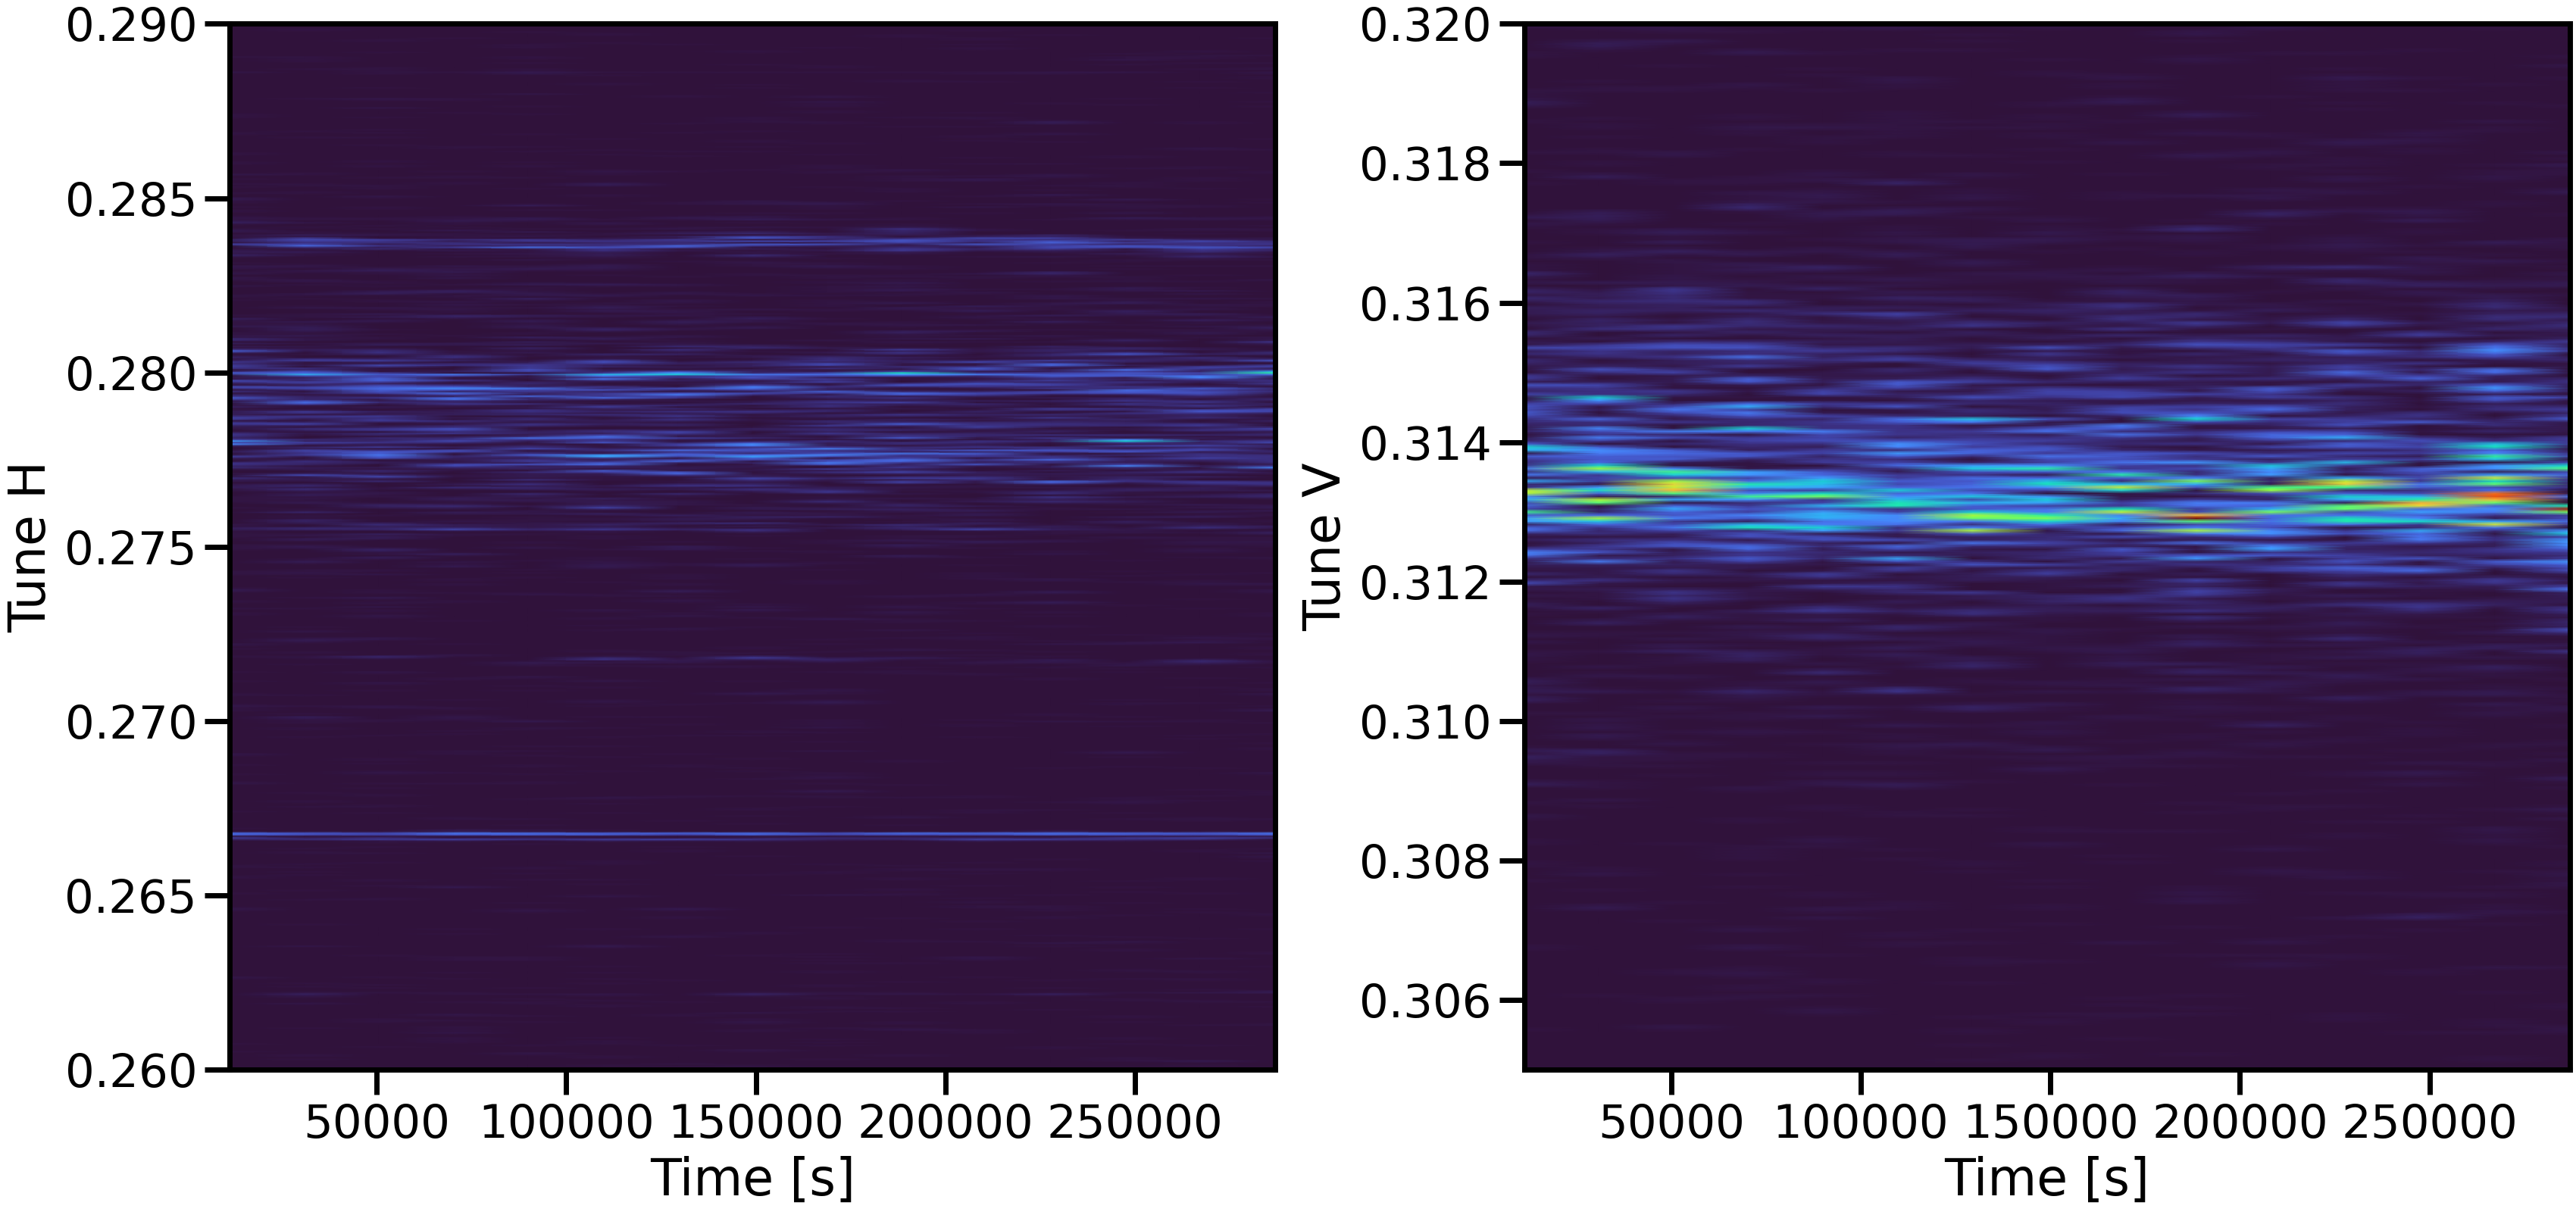
\includegraphics[width=.8\textwidth]{./images/spectrogram.png}
    \caption{Tune spectrogram obtained via BBQ system. Strong resonance lines can be seen above and
    below where the tune really is, causing the wrong frequency peak to be identified as the tune.}
    \label{fig:decapoles:chromaticity:spectrogram}
\end{figure}



% ========== Momentum Compaction Factor
\subsubsection{\review{Momentum Compaction Factor}}
\label{subsubsection:momentum_compaction_factor_studies}

Rather than a constant, the momentum compaction factor can be expressed as an
expansion, as detailed in~\cref{subsection:coordinates_systems:momentum_compaction_factor}.
The first terms are given by the following,

\begin{equation}
    \alpha_c = 
    \underbrace{\alpha_{c,0}}_{1^\text{st} \text{ order}}
    + \underbrace{\alpha_{c,1} \delta}_{2^\text{nd} \text{ order}}
    + \underbrace{\alpha_{c,2} \delta^2}_{3^\text{rd} \text{ order}}.
\end{equation}

The expression for $\delta$ at first and second order then reads,

\begin{equation}
    \begin{aligned}
        \delta &= -\frac{\Delta f_{RF}}{\alpha_{0} f_{RF}} && \Rightarrow \text{Order 1} \\
        \delta &= \frac{- \alpha_{0} f_{RF} + \sqrt{f_{RF} 
            \left(- 4 \Delta f_{RF} \alpha_{1} + \alpha_{0}^{2} f_{RF}\right)}}{2 \alpha_{1} f_{RF}}
            && \Rightarrow \text{Order 2} 
    \end{aligned}
\end{equation}

It is assumed that only the first term is relevant as the induced difference in chromaticity is
negligible as will be demonstrated later on.
\cref{fig:decapoles:chromaticity:momentum_compaction_factor} shows the non linearity of the momentum
compaction factor and its effect on the calculated $\delta$ via the previous formulas.

\begin{figure}[tbh]
    \centering
    \begin{subfigure}[t]{0.48\textwidth}
        \centering
        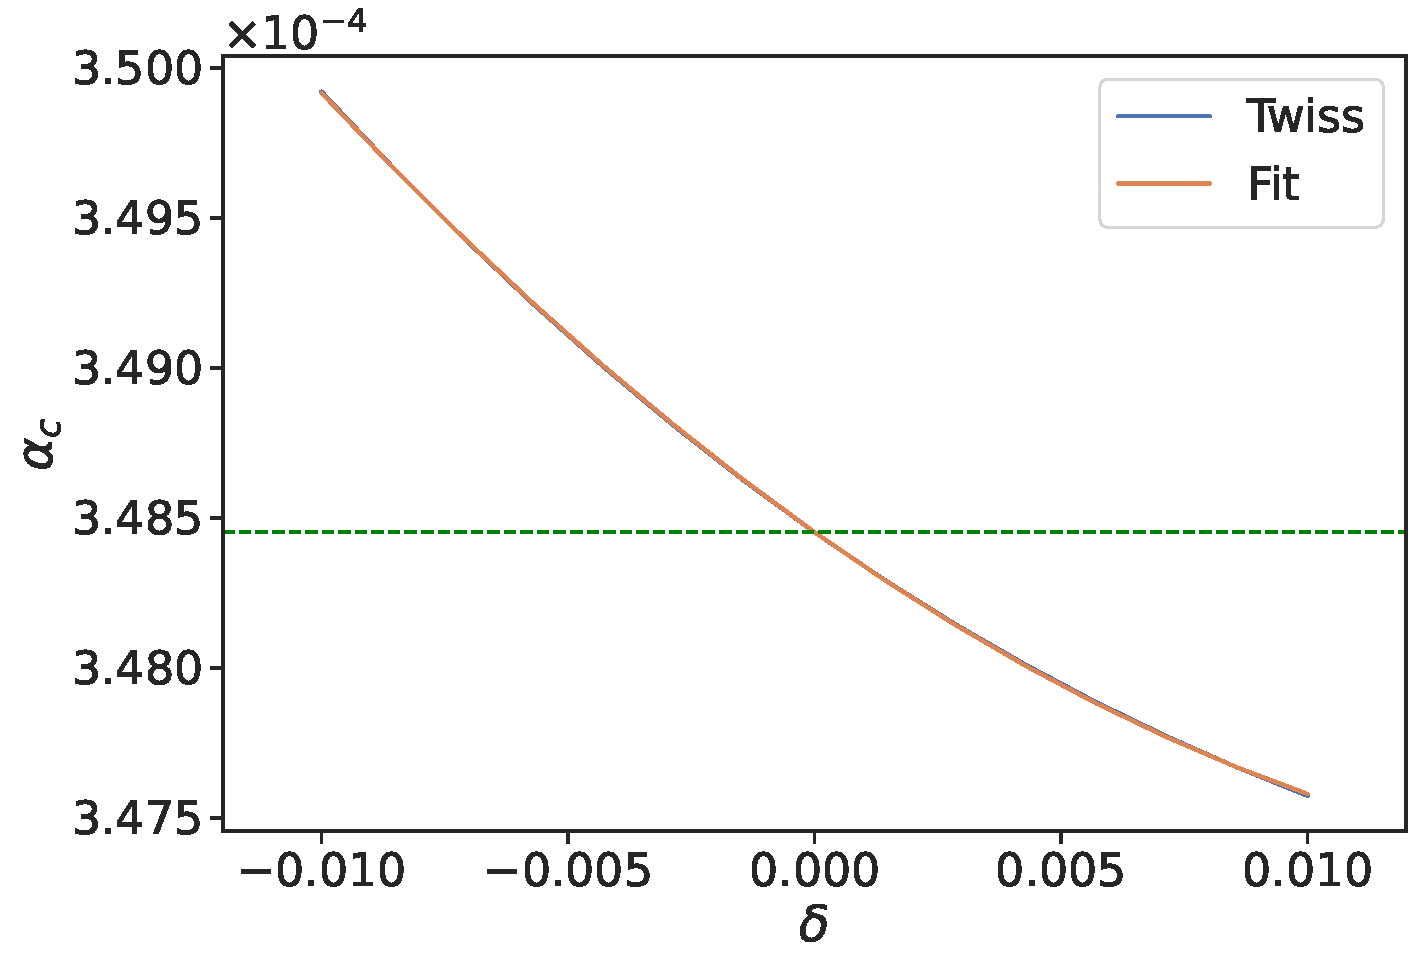
\includegraphics[width=\textwidth]{images/higher_order_momentum_compaction_factor.pdf}
        \caption{Non-linear fit of $\alpha_c$ obtained via an evaluation at discrete $\delta$ in
        MAD-X. The green line represents a constant $\alpha_c = \alpha_{c,0}$.}
    \end{subfigure}
    \hfill
    \begin{subfigure}[t]{0.48\textwidth}
        \centering
        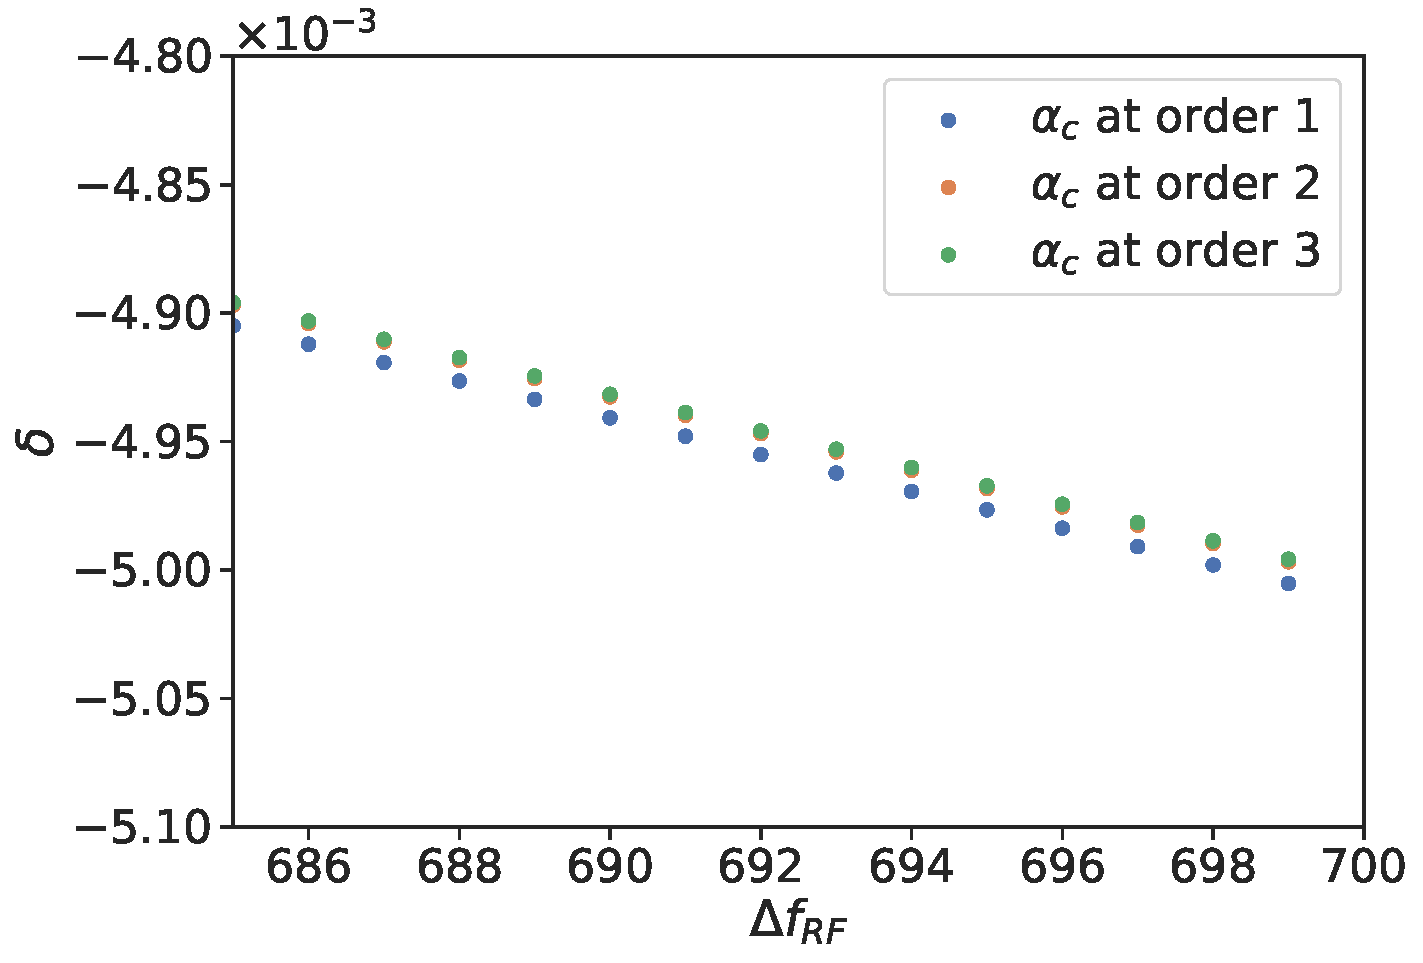
\includegraphics[width=\textwidth]{images/delta_vs_frf_alpha_c.pdf}
        \caption{Divergence of the momentum offset when considering higher $\alpha_c$ orders with
        large RF trims.}
    \end{subfigure}
    \caption{Non linearity of $\alpha_c$ and its effect on the computed $\delta$ via RF trims. The
    simulations are done at injection energy of 450GeV.}
    \label{fig:decapoles:chromaticity:momentum_compaction_factor}
\end{figure}

It is observed that while clearly depending on higher orders, the momentum compaction factor only
has a small impact on the calculated $\delta$.
\cref{fig:decapoles:chromaticity:momentum_compaction_factor_chroma_meas} shows a real-life 
measurement, comparing the fit of the chromaticity function with various $\delta$, computed up to
the third order of $\alpha_c$.

\begin{figure}[tbh]
    \centering
    \begin{subfigure}[t]{0.48\textwidth}
        \centering
        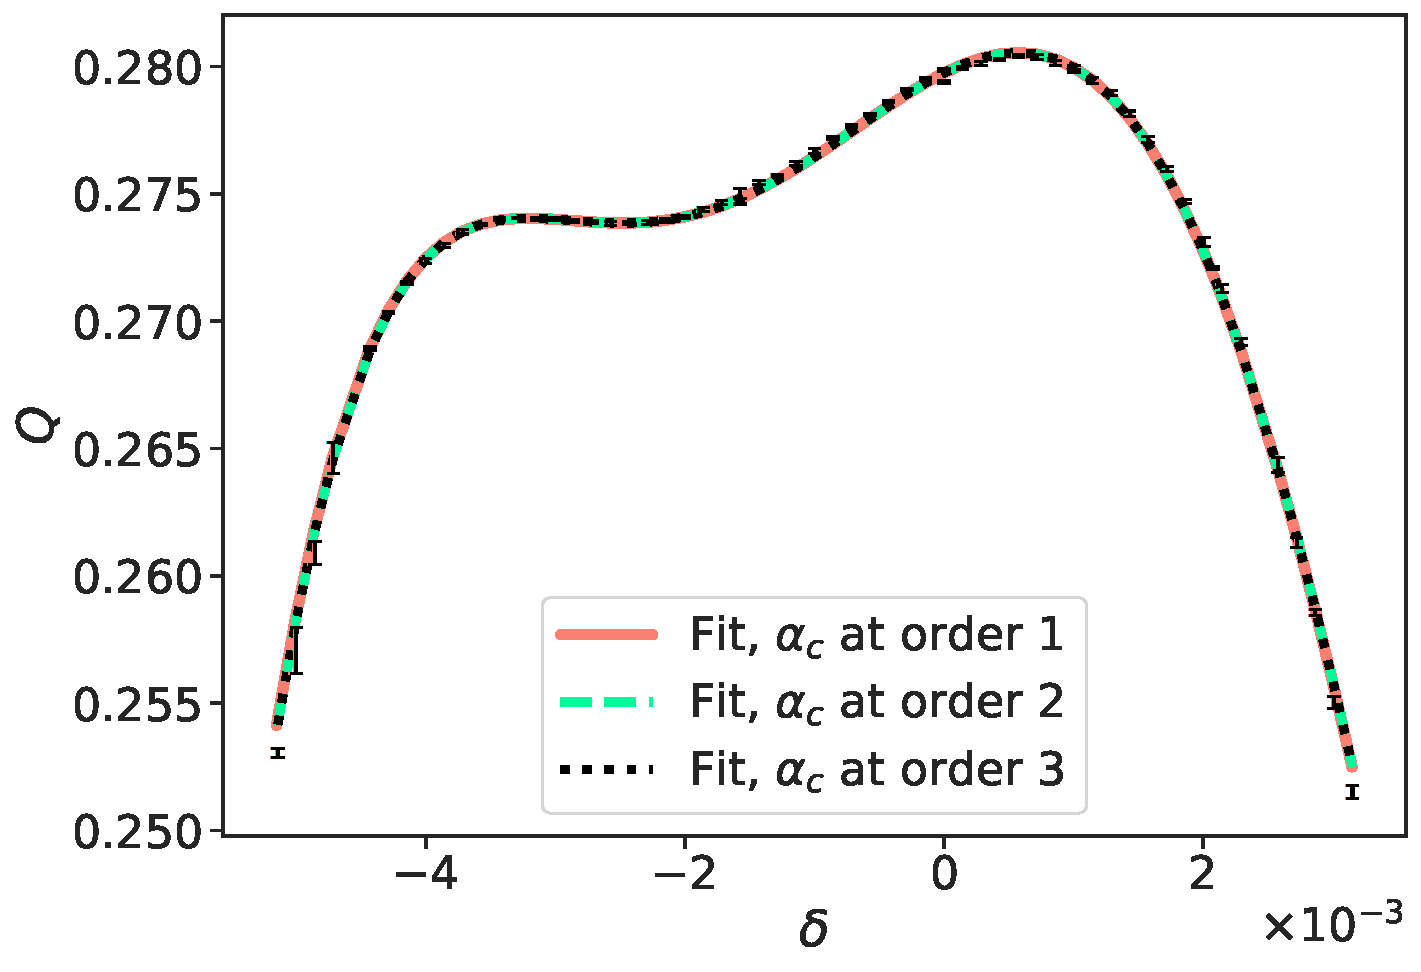
\includegraphics[width=\textwidth]{images/chroma_function_alpha_c.pdf}
        \caption{Fit of the chromaticity function at the $5^{\text{th}}$ order, considering the
        $\alpha_c$ expansion up to the third order.}
    \end{subfigure}
    \hfill
    \begin{subfigure}[t]{0.48\textwidth}
        \centering
        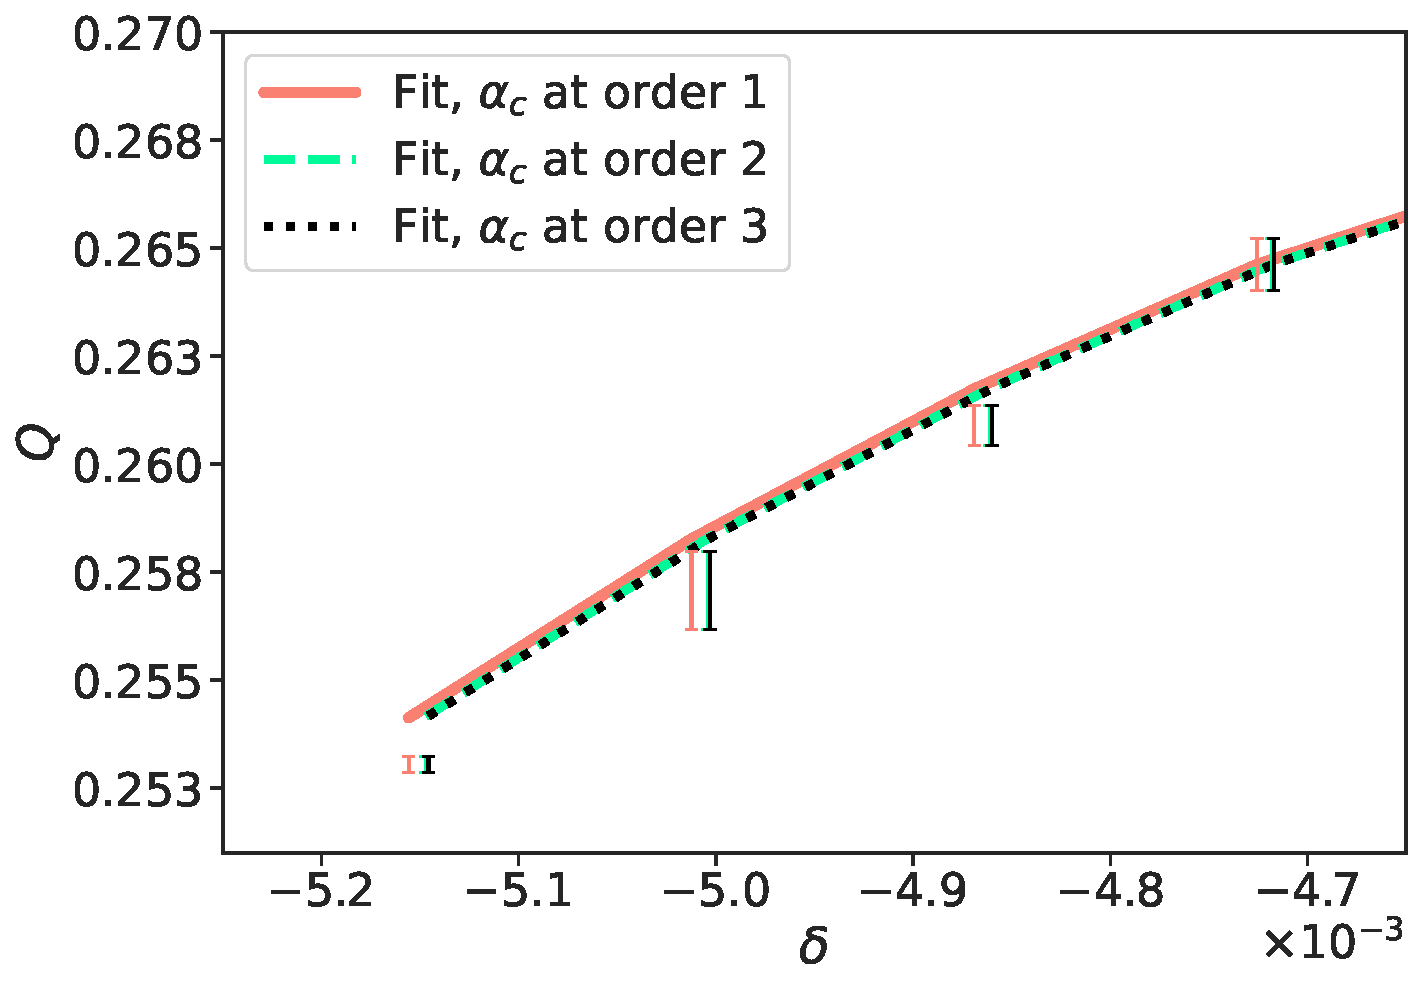
\includegraphics[width=\textwidth]{images/chroma_function_alpha_c_zoom.pdf}
        \caption{Zoom on one side of the fit. The difference between the second and third order
        is barely noticeable.}
    \end{subfigure}
    \caption{Fit of the chromaticity function considering several $\alpha_c$ orders.}
    \label{fig:decapoles:chromaticity:momentum_compaction_factor_chroma_meas}
\end{figure}

The fit of the chromaticity function is barely impacted when considering the higher orders of the 
momentum compaction factor. The different orders of the chromaticity are collected
in~\cref{table:decapoles:chromaticity:alpha_c_chroma}.
The higher order terms of $\alpha_c$ can thus be neglected and are not a source of higher
chromaticity orders.

\begin{table}[!htb]
    \centering
    \begin{tabular}{lrrr}
      \toprule
                  & \multicolumn{3}{c}{$\alpha_c$ order} \\
  %                \cmidrule{2-4}
      Chromaticity &  \multicolumn{1}{c}{1}  &  \multicolumn{1}{c}{2} &  \multicolumn{1}{c}{3} \\
      \midrule
      $Q^{(1)}$ & $ 2.52 \pm 0.03$ & $ 2.53 \pm 0.03$ & $ 2.53 \pm 0.03$ \\
      $Q^{(2)}$ & $-3.04 \pm 0.05$ & $-3.05 \pm 0.05$ & $-3.05 \pm 0.05$ \\
      $Q^{(3)}$ & $-4.75 \pm 0.03$ & $-4.75 \pm 0.03$ & $-4.75 \pm 0.03$ \\
      $Q^{(4)}$ & $-0.33 \pm 0.07$ & $-0.32 \pm 0.07$ & $-0.32 \pm 0.07$ \\
      $Q^{(5)}$ & $ 2.33 \pm 0.06$ & $ 2.36 \pm 0.06$ & $ 2.36 \pm 0.06$ \\
      \bottomrule
    \end{tabular}
    \caption{Chromaticity values obtained for the same measurement, depending on the order of the
    momentum compaction factor taken into account.}
    \label{table:decapoles:chromaticity:alpha_c_chroma}
\end{table}     

%----------------------------------------
%         Other dpp Measurements
\subsubsection{\review{Momentum Offset from Orbit}}

During machine operation, the momentum offset, derived from the orbit, used to be logged on the
servers. It was then possible to directly compute the chromaticity that way without having to use
the RF and the momentum compaction factor.
In 2016, measurements of the non-linear chromaticity were performed using the former method.
\cref{fig:very_high_orders:bare_chroma_2016} shows a comparison of the obtained non-linear 
chromaticity from both methods, while \cref{table:very_high_orders:bare_chroma_2016} shows a
numerical comparison. Results being similar, is it deemed that both methods are reliable to measure
the non-linear chromaticity in the LHC.


\begin{table}[!htb]
    \centering
    \begin{tabular}{lrrrr}
        \toprule
              & \multicolumn{2}{c}{$\delta$ via RF}  &  \multicolumn{2}{c}{$\delta$ via orbit} \\
        Plane & \multicolumn{1}{c}{$Q'' [10^3]$}     & \multicolumn{1}{c}{$Q''' [10^6]$} & \multicolumn{1}{c}{$Q'' [10^3]$} & \multicolumn{1}{c}{$Q''' [10^6]$}\\
        \midrule
        Beam 1 &&&& \\
        \hspace{2mm}X & $-0.64 \pm 0.01$ & $ 3.00 \pm 0.04$   & $-0.62 \pm 0.01$ & $ 2.91 \pm 0.04$ \\
        \hspace{2mm}Y & $-0.17 \pm 0.01$ & $-2.12 \pm 0.04$   & $-0.14 \pm 0.01$ & $-2.09 \pm 0.04$ \\
        Beam 2 &&&& \\
        \hspace{2mm}X & $-1.18 \pm 0.02$ & $ 2.89 \pm 0.06$   & $-1.23 \pm 0.03$ & $ 3.13 \pm 0.11$ \\
        \hspace{2mm}Y & $ 0.18 \pm 0.02$ & $-1.95 \pm 0.05$   & $ 0.20 \pm 0.02$ & $-2.02 \pm 0.06$ \\
        \bottomrule
    \end{tabular}
    \caption{Comparison of the chromaticity values obtained for the same measurement via two
    different methods to acquire $\delta$.}
    \label{table:very_high_orders:bare_chroma_2016}
  \end{table}


\begin{figure}[H]
    \begin{subfigure}{0.49\textwidth}
        \centering
        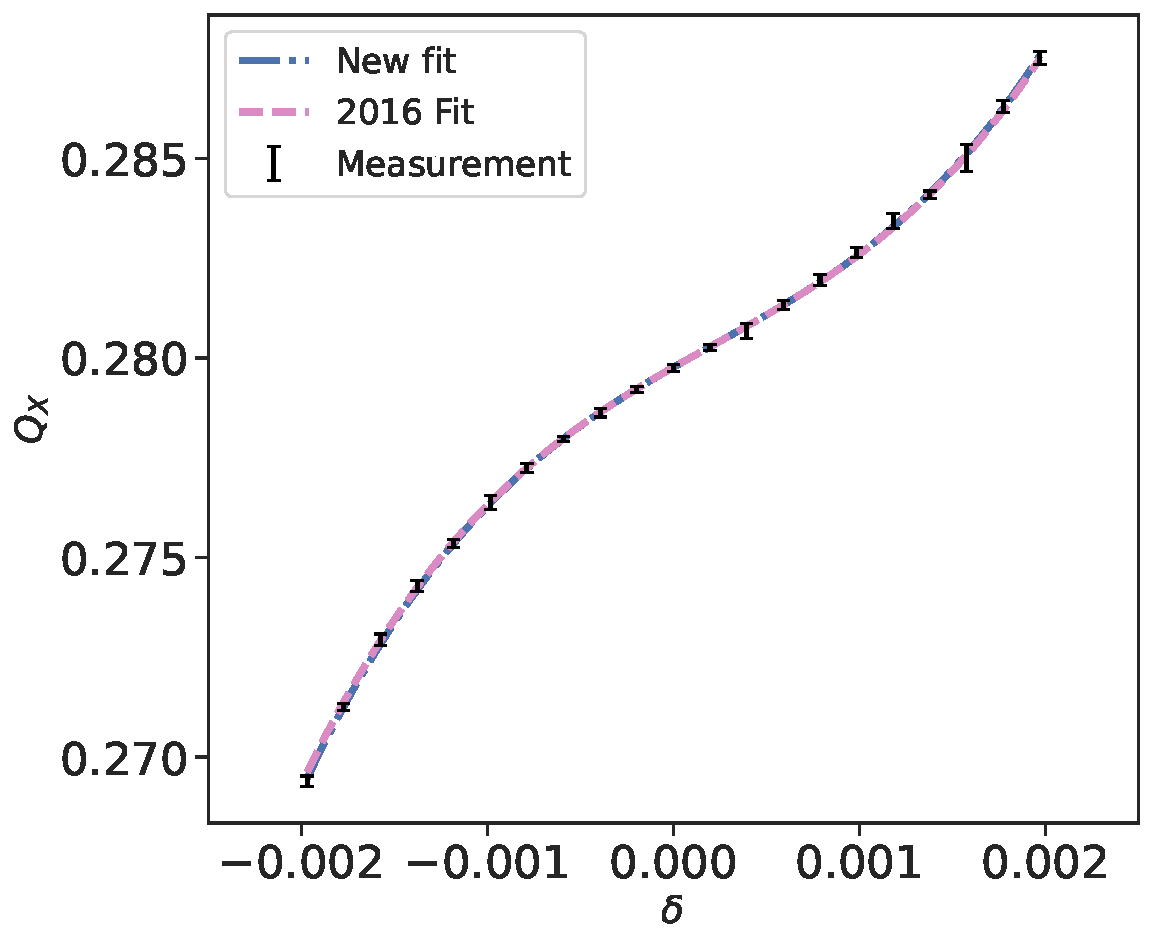
\includegraphics[width=\textwidth]{./images/chromaticity_2016/B1_qx.pdf}
        \caption{$Q_x$ Beam 1}
        \label{}
    \end{subfigure}
    \hfill
    \begin{subfigure}{0.49\textwidth}
        \centering
        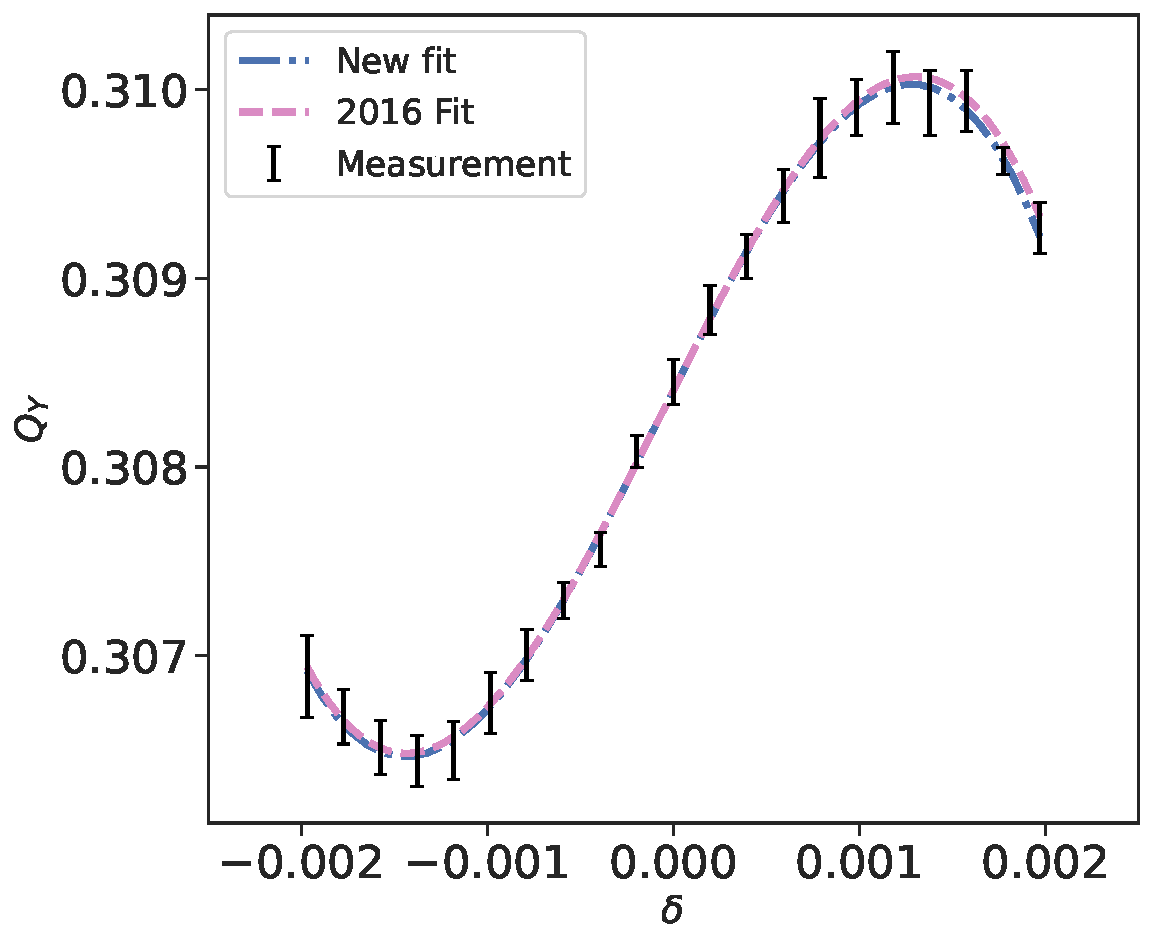
\includegraphics[width=\textwidth]{./images/chromaticity_2016/B1_qy.pdf}
        \caption{$Q_y$ Beam 1}
        \label{}
    \end{subfigure}
    %
    \\
    %
    \begin{subfigure}{0.49\textwidth}
        \centering
        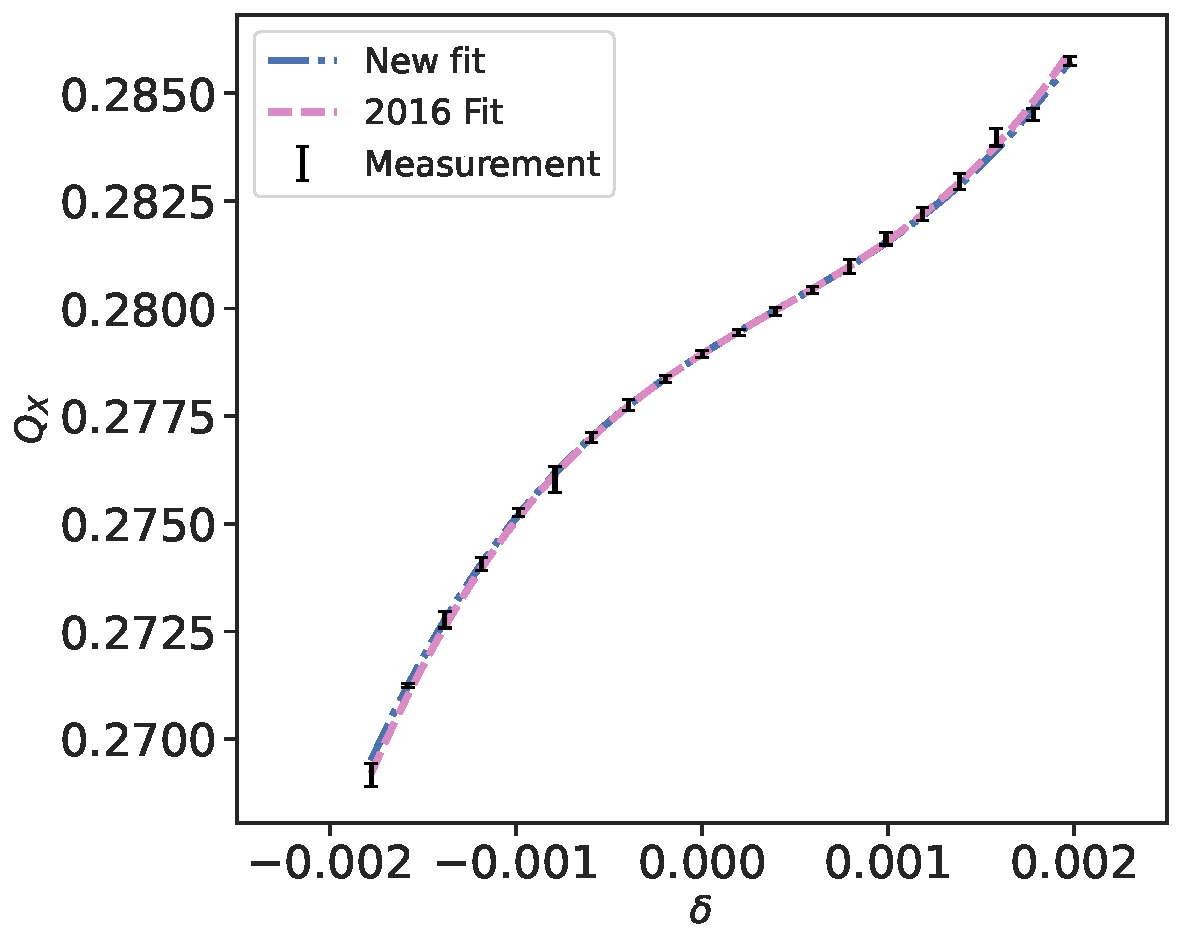
\includegraphics[width=\textwidth]{./images/chromaticity_2016/B2_qx.pdf}
        \caption{$Q_x$ Beam 2}
        \label{}
    \end{subfigure}
    \hfill
    \begin{subfigure}{0.49\textwidth}
        \centering
        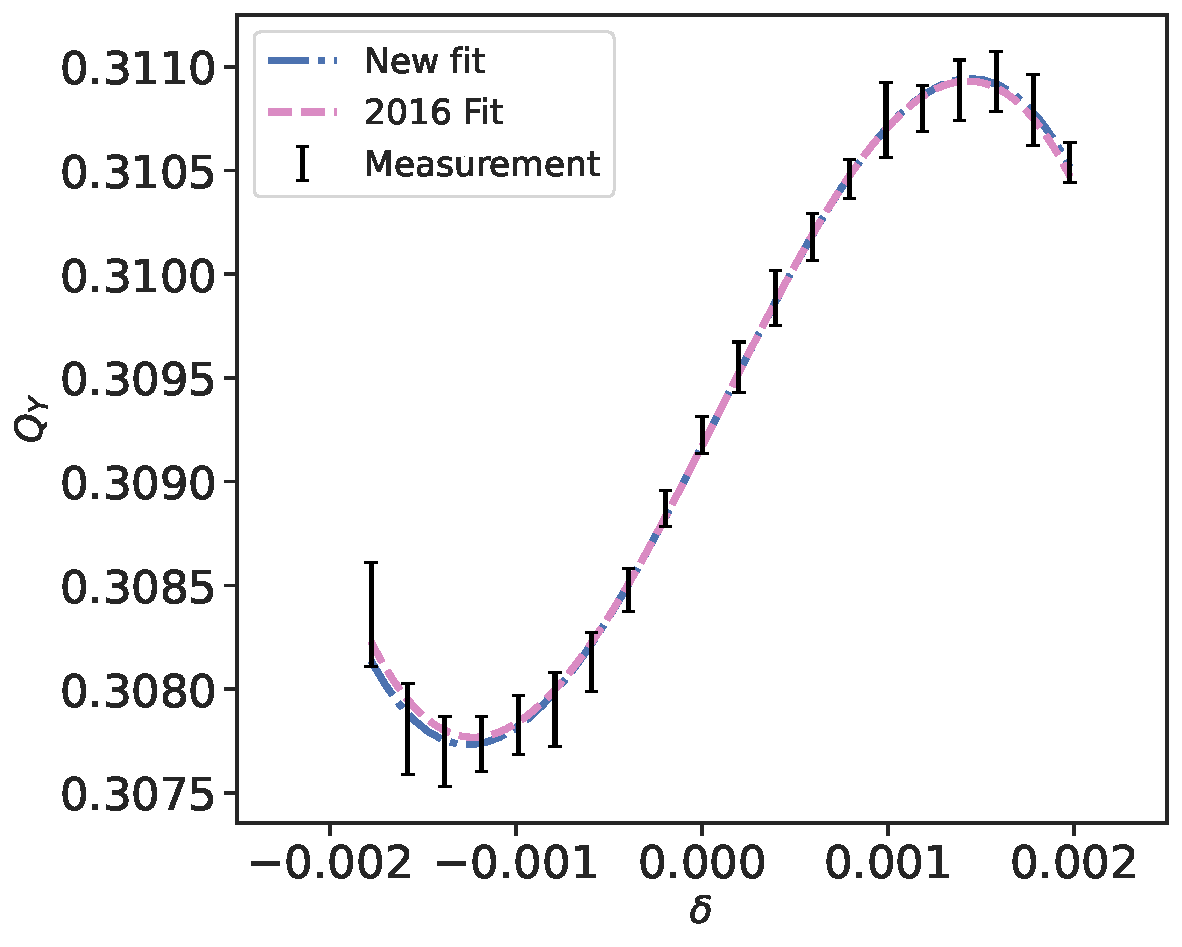
\includegraphics[width=\textwidth]{./images/chromaticity_2016/B2_qy.pdf}
        \caption{$Q_y$ Beam 2}
        \label{}
    \end{subfigure}
    \caption{Comparison of the non-linear chromaticity fit obtained from the computed momentum
    offset via the RF in 2022 and from the logged values in 2016.}
    \label{fig:very_high_orders:bare_chroma_2016}
\end{figure}


%----------------------------------------
%        Performed Measurements
%----------------------------------------
\subsection{\review{Measurements}}

In order to assess the correctness of the observation of higher chromaticity orders, measurement
repeatability is needed. Two measurements were thus take in 2022, with different configurations
pertaining to the correction of the second and third order chromaticities $Q''$ and $Q'''$. 
The first one used the nominal correction strengths for octupole and decapole corrector magnets,
derived from magnetic measurements, where the second one used beam-based corrections for the same
elements, computed from the previous measurement.
More measurements were taken during 2024's commissioning with new optics for the same reasons, to
minimize the second and third order chromaticities. Three measurements were taken: with nominal
corrections, after having corrected $Q'''$  and then $Q''$. The introduced new optics mainly changed
the powering of the triplets at the IPs and are not expected to have a considerable impact on the
chromaticity. 

\cref{table:high_orders:dpp_ranges} shows a summary of those measurements with their respective 
achieved momentum offset ranges. While the 2024 measurements achieved greater ranges than the
previous ones, those were restricted during analysis to allow suitable comparisons.

\begin{table}[!htb]
  \centering
  \begin{tabular}{lllcc}
    \toprule
    Number & Year & Corrections      & $\delta$ min. $[\times 10^{-3}]$ & $\delta$ max. $[\times 10^{-3}]$  \\
    \midrule
    1 & 2022 & Nominal          & $-3.15$ & $3.01$  \\
    2 & 2022 & $Q''$ \& $Q'''$  & $-3.15$ & $3.72$  \\
    3 & 2024 & Nominal          & $-5.15$ & $3.15$  \\
    4 & 2024 & $Q'''$           & $-3.44$ & $4.87$  \\
    5 & 2024 & $Q''$ \& $Q'''$  & $-3.86$ & $4.44$  \\
    \bottomrule
  \end{tabular}
  \caption{Performed chromaticity measurements with their respective momentum offset ranges.}
  \label{table:high_orders:dpp_ranges}
\end{table}

In order to stay consistent, the horizontal and vertical tunes were respectively set to $Q_x = 0.28$
and $Q_y = 0.31$ for both measurements. The linear chromaticity $Q'$ is set to a small value, around
$2$, to avoid large tune shifts throughout the scan.
All measurements were performed during LHC's beam commissioning, as part of the measurements and
corrections performed after technical or long shutdowns.


%----------------------------------------
%           First Measurement
\subsubsection{\review{First Observation}}

The first observation of higher order chromaticity was done with the octupolar and decapolar
correctors \textit{MCO} and \textit{MCD} set to their nominal settings. Those are aimed at
correcting $Q''$ and $Q'''$, as previously described in \cref{chapter:decapoles}.
Results of this initial measurement are shown in \cref{tab:high_orders:chroma_fidel}. Lower order
chromaticities such as $Q'$ and $Q''$ are consistent with measurements done during the previous 
Run~\cite{maclean_commissioning_2016}.

\begin{table}[!htb]
    \centering
    \begin{tabular}{lrrrr}
    \toprule
         Plane & $Q^{(2)} [10^3]$ & $Q^{(3)} [10^6]$ & $Q^{(4)} [10^9]$ & $Q^{(5)} [10^{12}]$ \\
    \midrule
        Beam 1 &              &               &              & \\
        \hspace{2mm}X         & $-2.44 \pm 0.02$ & $-3.36 \pm 0.04$ & $-0.56 \pm 0.02 $ & $ 1.20 \pm 0.07$ \\
        \hspace{2mm}Y         & $ 0.97 \pm 0.02$ & $ 1.62 \pm 0.05$ &$  0.15 \pm 0.03$ & $-0.88 \pm 0.09$ \\
        Beam 2 &              &                &                & \\
        \hspace{2mm}X         & $-2.45 \pm 0.03$ & $-2.72 \pm 0.08$ & $-1.00 \pm 0.05 $ & $ 0.15 \pm 0.14$ \\
        \hspace{2mm}Y         & $ 0.79 \pm 0.03$ & $1.54 \pm 0.06 $ & $ 0.24 \pm 0.04 $ & $-0.74 \pm 0.13$ \\
    \bottomrule
    \end{tabular}
    \caption{Terms of the high order chromaticity obtained during Run~3's commissioning in 2022,
    with nominal corrections.}
    \label{tab:high_orders:chroma_fidel}
  \end{table}

Due to the RF-scan method, the momentum offset crosses zero several times during the measurement.
Negligible change in tune at this point makes it possible to determine that the tune drift through
the measurement is of no consequence.
This measurement was performed after an extended period at injection energy, where the decay of the
sextupolar fields is small and not causing any change in the first order chromaticity. The fitted
curve for the chromaticity function is shown in \cref{fig:high_orders:chroma_before_correction}. 
It is clear that a higher order polynomial is beneficial to the fit, as discussed further in
\cref{subsection:q4q5_quality}.

\begin{figure}[H]
    \begin{subfigure}{0.49\textwidth}
        \centering
        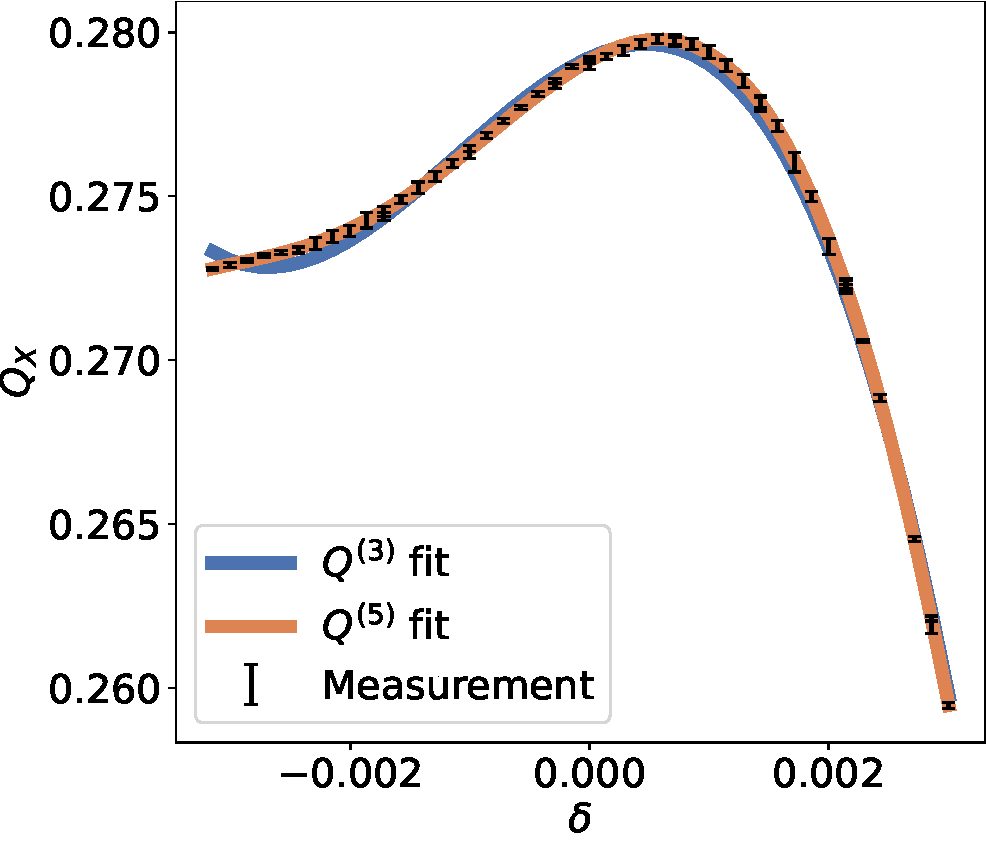
\includegraphics[width=\textwidth]{./images/higher_orders/fidel_chroma/Beam1_Qx.pdf}
        \caption{$Q_x$ Beam 1}
        \label{}
    \end{subfigure}
    \hfill
    \begin{subfigure}{0.49\textwidth}
        \centering
        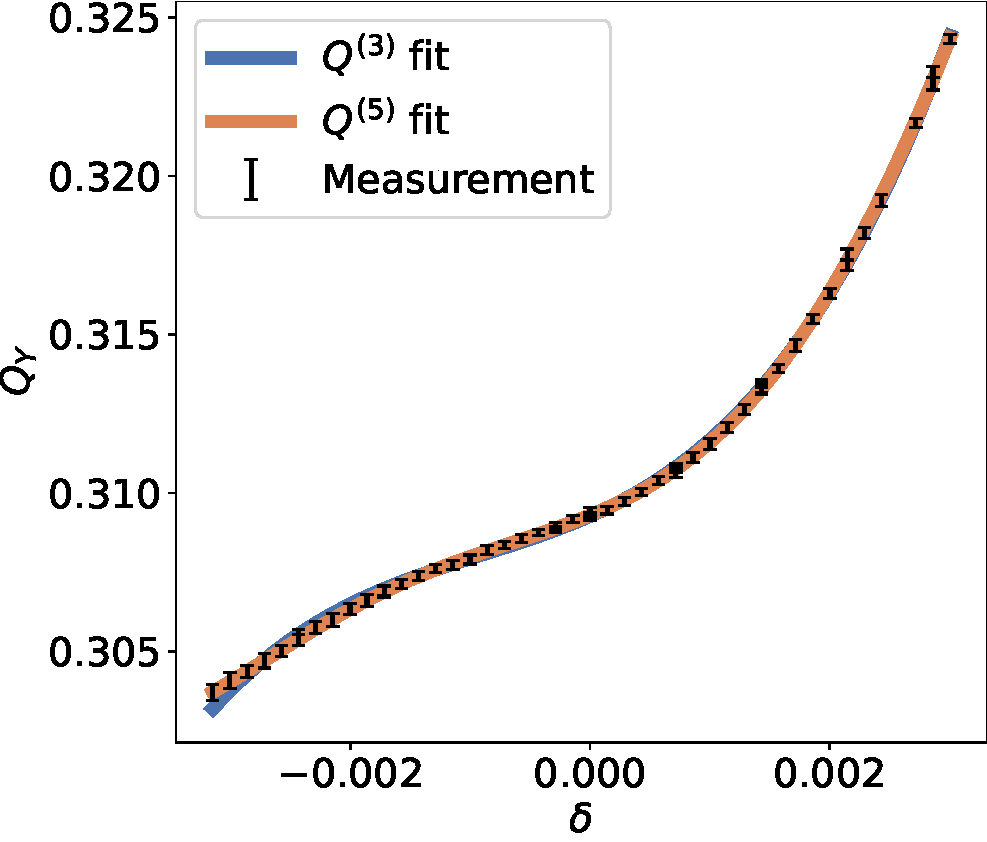
\includegraphics[width=\textwidth]{./images/higher_orders/fidel_chroma/Beam1_Qy.pdf}
        \caption{$Q_y$ Beam 1}
        \label{}
    \end{subfigure}
    %
    \\
    %
    \begin{subfigure}{0.49\textwidth}
        \centering
        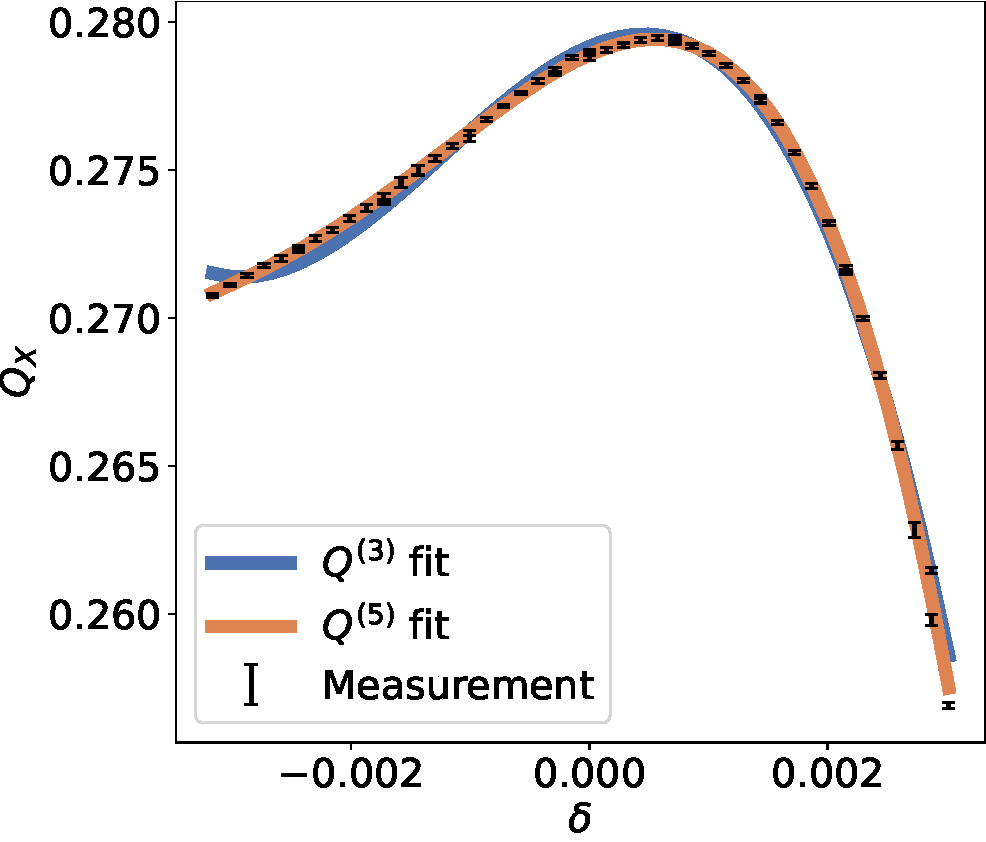
\includegraphics[width=\textwidth]{./images/higher_orders/fidel_chroma/Beam2_Qx.pdf}
        \caption{$Q_x$ Beam 2}
        \label{}
    \end{subfigure}
    \hfill
    \begin{subfigure}{0.49\textwidth}
        \centering
        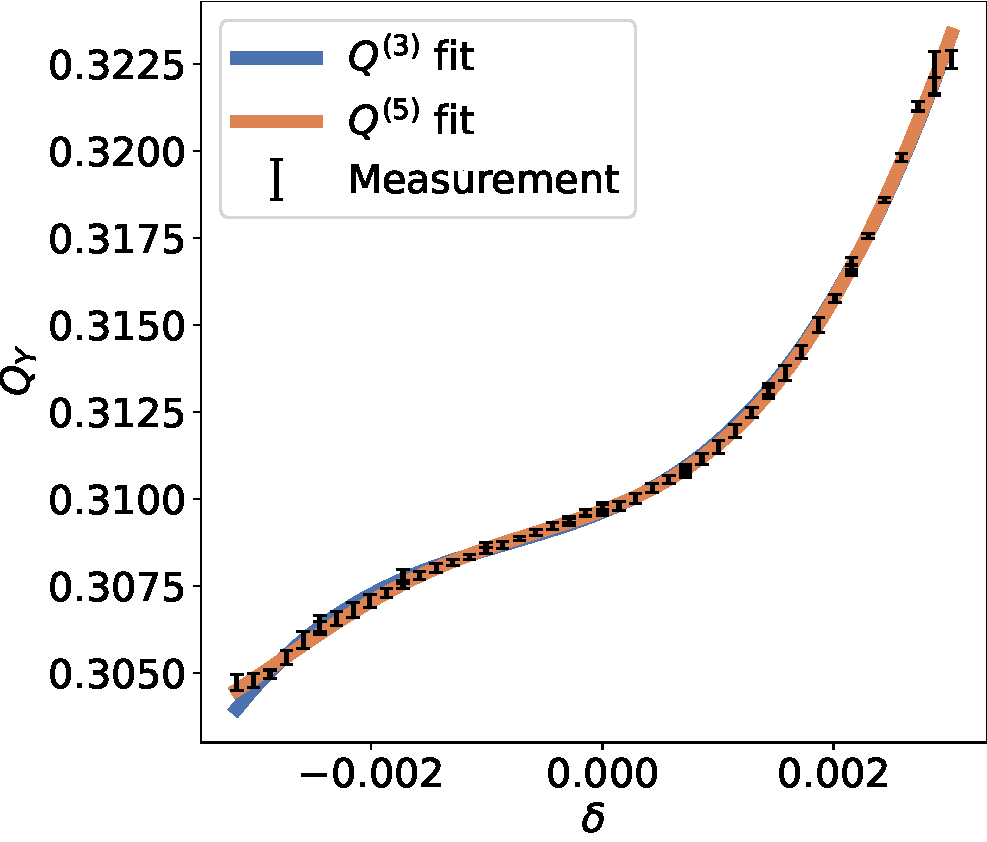
\includegraphics[width=\textwidth]{./images/higher_orders/fidel_chroma/Beam2_Qy.pdf}
        \caption{$Q_y$ Beam 2}
        \label{}
    \end{subfigure}
    \caption{Measurement of higher order chromaticity terms with nominal corrections used
    during operation. Fits are up to the third and fifth order.}
    \label{fig:high_orders:chroma_before_correction}
\end{figure}

Previous studies of chromaticity in the LHC only considered fits up to the third order.
Expanding the fits to the fifth order increases the $Q'''$ estimate and improves the fit quality. 
Accurately measuring the third order chromaticity is essential for its correction, making it
important to consider the higher orders.



%----------------------------------------
%       Varying Configurations
\subsubsection{\review{Varying Configurations}}

The five previously introduced measurements were performed with very different configurations for
the octupolar and decapolar correctors. \cref{tab:high_orders:mcdo_values_corr} shows the strengths
applied on every circuit for each correction scheme, in 2022. The correction is called 
\textit{global} as all correctors are trimmed uniformly. The 2024 corrections are similar in order
of magnitude.
\cref{fig:high_orders:comparison_2022_2024} shows the measurements and fit of some of these
measurements, to highlight their differences.

\begin{table}[H]
  \centering
  \begin{tabular}{lll}
  \toprule
    Beam  &    $K_4 [\mathrm{m}^{-4}]$      &  $K_5 [\mathrm{m}^{-5}]$  \\
  \midrule
      1   &   +3.2973    &  +1610   \\
      2   &   +2.1716    &  +1618   \\
  \bottomrule
  \end{tabular}
  \caption{Corrections applied on top of the nominal octupolar and decapolar correctors strengths in
  2022 for the $Q''$ and $Q'''$ corrections.}
  \label{tab:high_orders:mcdo_values_corr}
\end{table}

\begin{figure}[H]
  \centering
  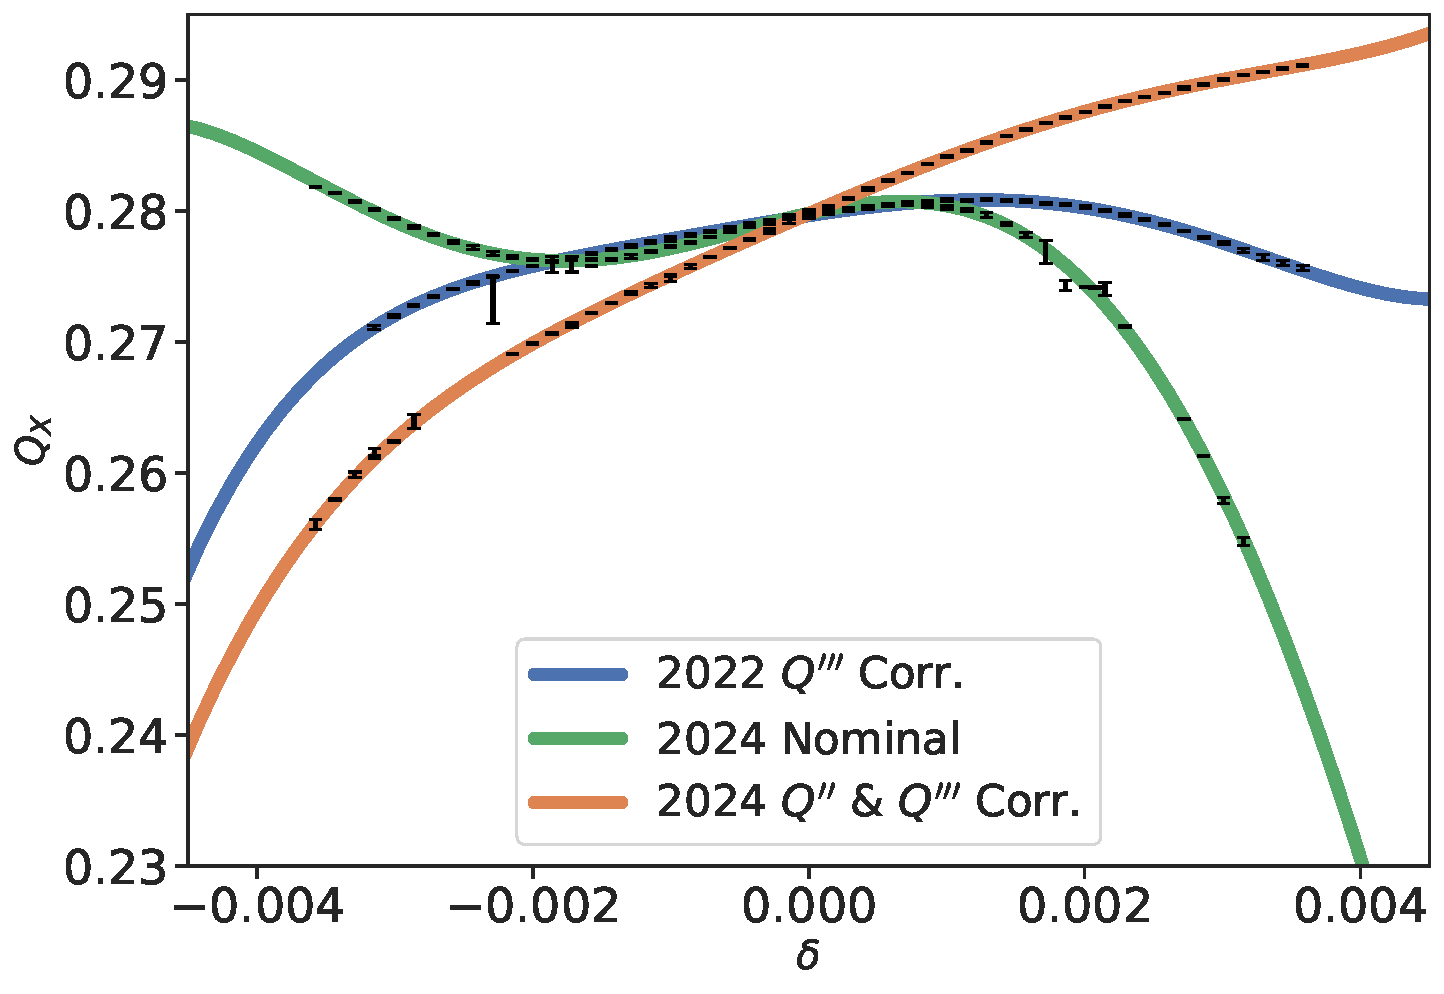
\includegraphics[width=0.7\textwidth]{./images/chromaticity_2024_vs_2022/chroma_comparison_B1_X.pdf}
  \caption{Selection of horizontal chromaticity measurements performed with varying configurations
  of the octupolar and decapolar correctors for Beam 1 during the commissionings of 2022 and 2024.}
  \label{fig:high_orders:comparison_2022_2024}
\end{figure}

A summary of the measured chromaticity orders is given in \cref{fig:high_oders:all_values}.
The first measurement in the horizontal plane of Beam 2 showed a high correlation between $Q^{(4)}$ and
$Q^{(5)}$, making the fit less reliable and is not included. The last measurement for the vertical
plane experienced some tune drift, making the fit impossible and is therefore not included for both
beams.

% The average is weighted by the errors
\begin{table}
  \centering
  \small
  \begin{tabular}{lrrrrr}
    \toprule
    Axis & Meas. & $Q''$ & $Q'''$ & $Q^{(4)}$ & $Q^{(5)}$ \\
    \midrule
    Horizontal &&&&&\\
    \hspace{2mm}Beam 1 & 1 & $-2.44\pm0.02$ & $-3.37\pm0.04$ & $-0.56\pm0.02$ & $ 1.21\pm0.07$ \\
                       & 2 & $-0.61\pm0.01$ & $-1.00\pm0.03$ & $-0.62\pm0.02$ & $ 1.19\pm0.05$ \\
                       & 3 & $-2.01\pm0.05$ & $-4.49\pm0.10$ & $-0.58\pm0.07$ & $ 1.34\pm0.18$ \\
                       & 4 & $-1.46\pm0.03$ & $-0.29\pm0.06$ & $-0.43\pm0.04$ & $ 1.09\pm0.10$ \\
                       & 5 & $-0.33\pm0.01$ & $-0.31\pm0.03$ & $-0.59\pm0.01$ & $ 0.75\pm0.04$ \\
                       & \textbf{Avg.}&     &                & $-0.56\pm0.07$ & $ 1.12\pm0.20$ \\%[0.5em]
                       \hdashline\noalign{\vskip 1ex}
    \hspace{2mm}Beam 2% & 1 & $-2.45\pm0.03$ & $-2.72\pm0.08$ & $-1.00\pm0.05$ & $ 0.15\pm0.14$ \\  % bad correlation for n°1
                       & 2 & $-0.85\pm0.01$ & $-0.66\pm0.03$ & $-0.57\pm0.02$ & $ 1.09\pm0.06$ \\
                       & 3 & $-2.93\pm0.05$ & $-4.40\pm0.08$ & $-0.53\pm0.08$ & $ 1.66\pm0.16$ \\
                       & 4 & $-2.21\pm0.02$ & $-0.00\pm0.03$ & $-0.46\pm0.02$ & $ 1.18\pm0.05$ \\
                       & 5 & $-0.53\pm0.02$ & $-0.09\pm0.03$ & $-0.57\pm0.02$ & $ 0.98\pm0.05$ \\
                       & \textbf{Avg.}&     &                & $-0.53\pm0.04$ & $ 1.23\pm0.26$ \\%[0.5em]
                       \midrule
    Vertical &&&&&\\
    \hspace{2mm}Beam 1 & 1 & $ 0.97\pm0.02$ & $ 1.62\pm0.05$ & $ 0.15\pm0.03$ & $-0.88\pm0.09$ \\
                       & 2 & $-0.23\pm0.01$ & $ 0.13\pm0.02$ & $ 0.09\pm0.02$ & $-0.60\pm0.03$ \\
                       & 3 & $ 0.83\pm0.02$ & $ 1.97\pm0.03$ & $ 0.29\pm0.02$ & $-0.68\pm0.05$ \\
                       & 4 & $ 0.62\pm0.01$ & $-0.18\pm0.03$ & $ 0.00\pm0.02$ & $-0.56\pm0.05$ \\
                       %& 5 & $-0.28\pm0.02$ & $-0.25\pm0.04$ & $ 0.28\pm0.02$ & $-0.12\pm0.05$ \\
                       & \textbf{Avg.}&     &                & $ 0.13\pm0.11$ & $-0.68\pm0.12$ \\%[0.5em]
                       \hdashline\noalign{\vskip 1ex}
    \hspace{2mm}Beam 2 & 1 & $ 0.79\pm0.03$ & $ 1.54\pm0.06$ & $ 0.24\pm0.04$ & $-0.74\pm0.13$ \\
                       & 2 & $-0.29\pm0.01$ & $ 0.10\pm0.02$ & $ 0.13\pm0.02$ & $-0.58\pm0.04$ \\
                       & 3 & $ 0.89\pm0.02$ & $ 2.05\pm0.03$ & $ 0.32\pm0.03$ & $-0.73\pm0.06$ \\
                       & 4 & $ 0.60\pm0.02$ & $-0.14\pm0.03$ & $ 0.04\pm0.02$ & $-0.66\pm0.05$ \\
                       %& 5 & $-0.62\pm0.02$ & $-0.29\pm0.04$ & $ 0.29\pm0.02$ & $-0.19\pm0.06$ \\
                       & \textbf{Avg.}&     &                & $ 0.18\pm0.11$ & $-0.68\pm0.06$ \\%[0.5em]
    \bottomrule
  \end{tabular}
  \caption{Summary of the chromaticity values obtained from the measurements presented in
  \cref{table:high_orders:dpp_ranges}.}
  \label{fig:high_oders:all_values}
\end{table}



%----------------------------------------
%       Beam-Based Corrections
%\subsubsection{\todo{Beam-Based Corrections}}
%
%After having corrected the second and third order chromaticities via the octupolar and decapolar
%correctors, a second measurement was performed.
%A uniform trim on all the correctors of each class was applied for each beam, resulting in a global
%correction. A total of four circuits were unavailable for the octupoles, three for beam 1 and one
%for beam 2, resulting in larger corrections for beam 1. The corrections are applied on top of the
%nominal settings~\cite{maclean_commissioning_2016}.
%The applied delta is shown in \cref{tab:high_orders:mcdo_values_corr}.
%\cref{fig:high_orders:chroma_after_correction} shows the chromaticity function fitted to the 
%measured tune after the beam-based minimization of $Q''$ and $Q'''$, while
%\cref{tab:high_orders:chroma_table_after} shows the values of that chromaticity fit.
%
%\begin{table}[!htb]
%    \centering
%    \begin{tabular}{lll}
%    \toprule
%      Beam  &    $K_4 [\mathrm{m}^{-4}]$      &  $K_5 [\mathrm{m}^{-5}]$  \\
%    \midrule
%        1   &  +3.2973     &  +1610   \\
%        2   &   +2.1716    &  +1618   \\
%    \bottomrule
%    \end{tabular}
%    \caption{Corrections applied on top of the nominal octupole and decapole correctors strengths.}
%    \label{tab:high_orders:mcdo_values_corr}
%  \end{table}
%
%\begin{figure}[!htb]
%    \begin{subfigure}{0.49\textwidth}
%        \centering
%        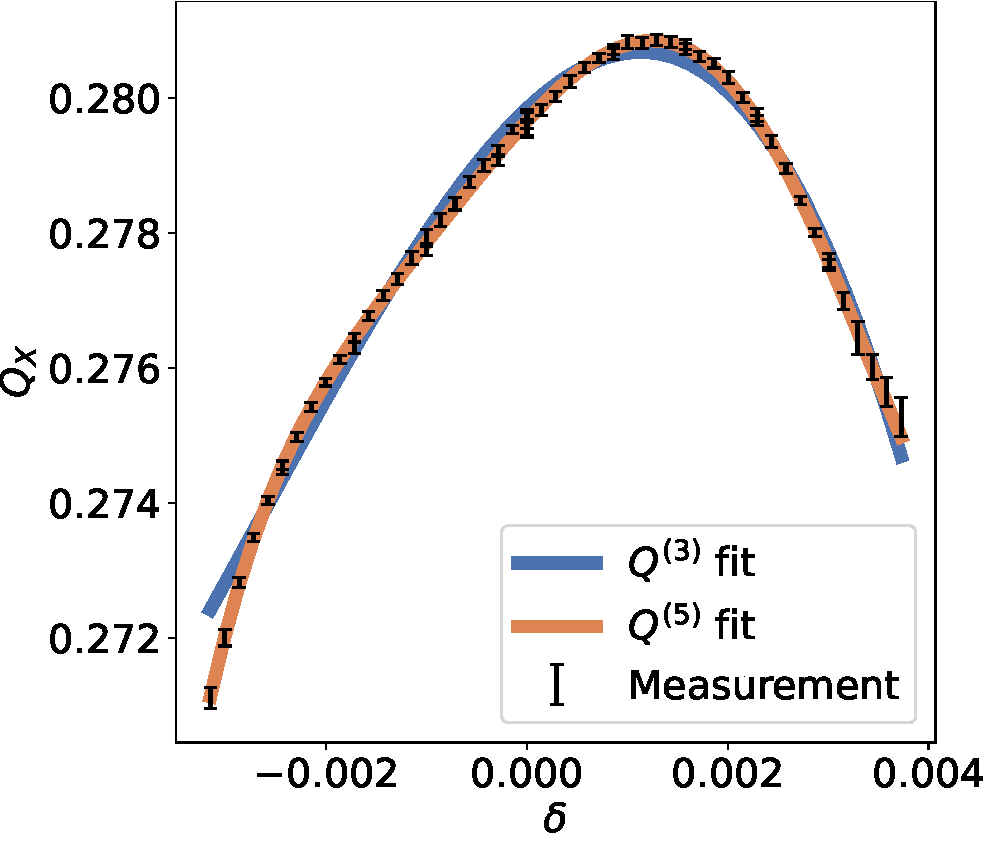
\includegraphics[width=\textwidth]{./images/higher_orders/bb_corrections_chroma/Beam1_Qx.pdf}
%        \caption{$Q_x$ Beam 1}
%        \label{}
%    \end{subfigure}
%    \hfill
%    \begin{subfigure}{0.49\textwidth}
%        \centering
%        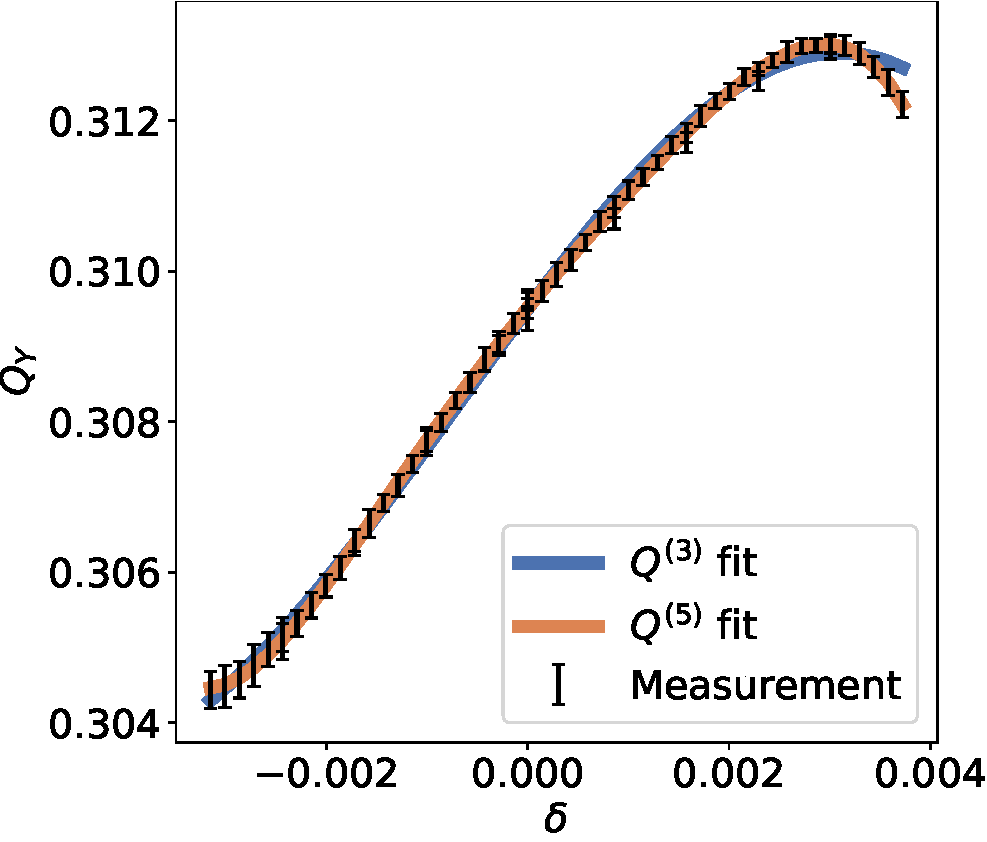
\includegraphics[width=\textwidth]{./images/higher_orders/bb_corrections_chroma/Beam1_Qy.pdf}
%        \caption{$Q_y$ Beam 1}
%        \label{}
%    \end{subfigure}
%    %
%    \\
%    %
%    \begin{subfigure}{0.49\textwidth}
%        \centering
%        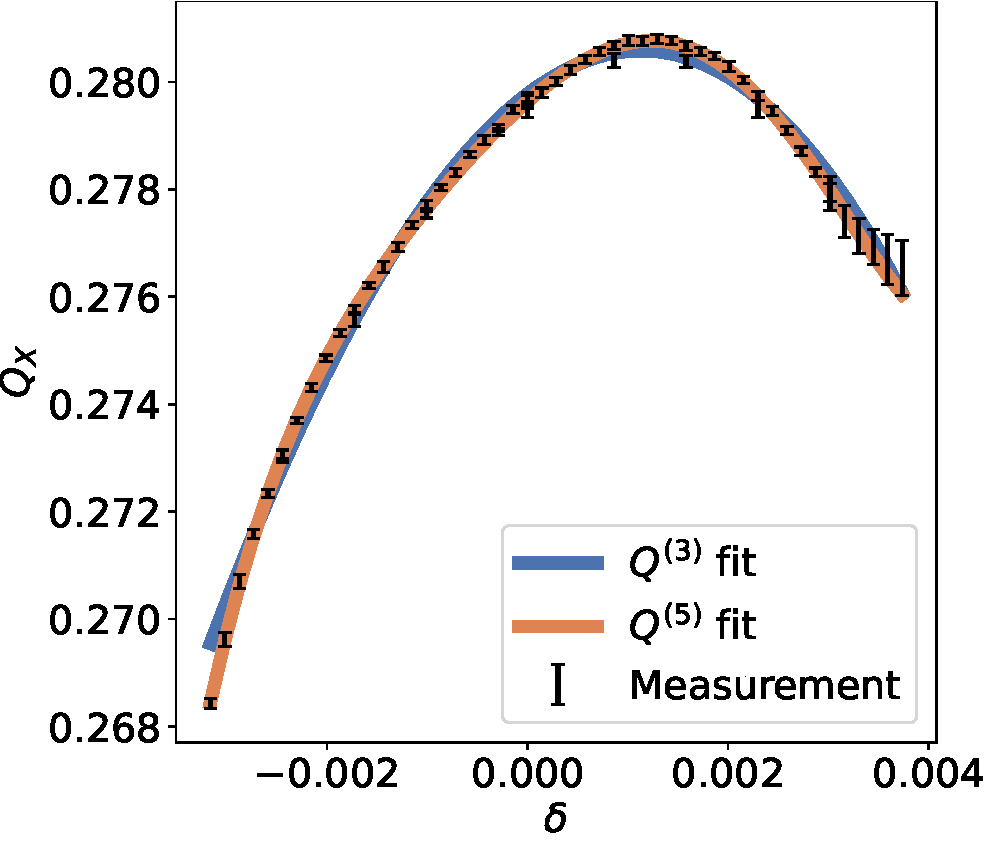
\includegraphics[width=\textwidth]{./images/higher_orders/bb_corrections_chroma/Beam2_Qx.pdf}
%        \caption{$Q_x$ Beam 2}
%        \label{}
%    \end{subfigure}
%    \hfill
%    \begin{subfigure}{0.49\textwidth}
%        \centering
%        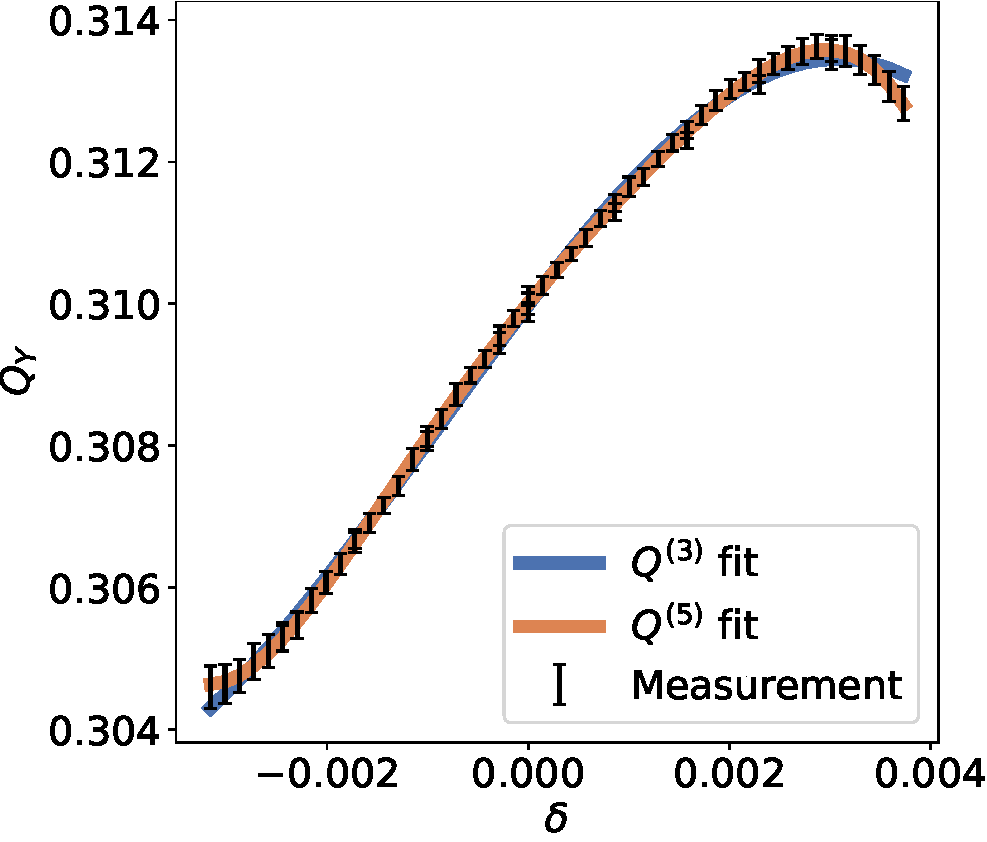
\includegraphics[width=\textwidth]{./images/higher_orders/bb_corrections_chroma/Beam2_Qy.pdf}
%        \caption{$Q_y$ Beam 2}
%        \label{}
%    \end{subfigure}
%    \caption{Measurement of high order chromaticity terms after application of $Q''$ and $Q'''$ 
%    beam-based corrections on octupolar and decapolar correctors.}
%    \label{fig:high_orders:chroma_after_correction}
%\end{figure}
%
%
%\begin{table}[!htb]
%    \centering
%    \begin{tabular}{lrrrr}
%      \toprule
%       Plane          & $Q^{(2)} [10^3]$ & $Q^{(3)} [10^6]$ & $Q^{(4)} [10^9]$ & $Q^{(5)} [10^{12}]$ \\
%      \midrule
%        Beam 1    &           &          &              &              \\
%        \hspace{2mm}X         & $-0.62 \pm 0.01$     & $-1.02 \pm 0.03$ & $-0.63 \pm 0.02$ &$  1.22 \pm 0.05$ \\
%        \hspace{2mm}Y         & $-0.24 \pm 0.01$     & $0.12 \pm 0.02 $&  $0.04 \pm 0.02 $& $-0.56 \pm 0.04 $\\
%        Beam 2    &           &&&     \\
%        \hspace{2mm}X         & $-0.85 \pm 0.01$     & $-0.64 \pm 0.03$ & $-0.58 \pm 0.02$ &$  1.07 \pm 0.06$ \\
%        \hspace{2mm}Y         & $-0.30 \pm 0.02$     & $0.14 \pm 0.03 $&  $0.16 \pm 0.02 $& $-0.66 \pm 0.05 $\\
%      \bottomrule
%    \end{tabular}
%    \caption{Terms of higher order chromaticity obtained during Run~3 commissioning in 2022,
%    with beam-based corrections for $Q''$ and $Q'''$.}
%    \label{tab:high_orders:chroma_table_after}
%\end{table}



%----------------------------------------
%             Fit Quality
%----------------------------------------
\subsubsection{\review{Fit Quality}}
\label{subsection:q4q5_quality}

The values measured for $Q^{(4)}$ and $Q^{(5)}$ are similar across the measurements, with
nominal and beam-based corrections performed with very different lower order chromaticity, and well 
separated in time.
This reproducibility with varying configurations gives confidence that the measured values are
robust. It is to be noted that one exception exists for the first measurement, the horizontal plane
of beam 2 showed a high correlation between the fourth and fifth order terms, making the fit less
reliable.

The reduced chi-square for the last measurement of 2022 for each fit order is detailed in
\cref{tab:high_orders:chisquare_quality}. While adding terms to the chromaticity function is
beneficial to the fit, it can be seen that the reduced chi-square does not substantially improve 
above the fifth order, indicating that such further orders are not warranted.
%Figure \ref{chroma_comparison} shows a comparison of the measured chromaticity before and after
%beam-based corrections for the horizontal axis of beam 1.

\begin{table}[H]
    \centering
    \begin{tabular}{lrrrr}
     \toprule
                  & \multicolumn{4}{c}{$\chi^2_\nu$} \\
      %\cmidrule{2-5}
        Plane     &   $Q^{(3)}$ &  $Q^{(4)}$ &   $Q^{(5)}$ &   $Q^{(6)}$  \\
      \midrule
        Beam 1    &   &   &   & \\
        % The commented out lines are from measurement with the regular BBQ data
        % The un-commented lines are from using the raw BBQ data
        %X         & 7.62  & 4.07 & 0.62 &\\             % regular
        %Y         & 0.72  & 0.57 & 0.15 &\\             % regular
        \hspace{2mm}X         & $17.9$  & $12.1$ & $1.8$ & $1.5$ \\         % raw bbq
        \hspace{2mm}Y         & $ 3.0$  & $2.2 $ & $0.7$ & $0.7 $\\          % raw bbq
        Beam 2    &    &    &   &\\
        %X         & 7.60  & 3.10 & 0.73 &\\             % regular
        %Y         & 0.48  & 0.46 & 0.16 &\\ \hline      % regular
        \hspace{2mm}X         & $17.3$ & $7.1$ & $1.8$ & $1.8$ \\           % raw bbq
        \hspace{2mm}Y         & $2.9 $ & $2.8$ & $1.0$ & $1.0$ \\            % raw bbq
      \bottomrule
    \end{tabular}
    \caption{Reduced $\chi^2$ values for each order of fit, taken from the second
    measurement of 2022, with $Q''$ and $Q'''$ beam-based corrections.}
    \label{tab:high_orders:chisquare_quality}
  \end{table}

%\begin{figure}[!ht]
%    \centering
%    \includegraphics[width=1\columnwidth]{images/comparison_b1x.png}
%    \caption{Comparison of the chromaticity function with nominal and beam-based corrections.}
%    \label[type]{chroma_comparison}
%\end{figure}
